% This is samplepaper.tex, a sample chapter demonstrating the
% LLNCS macro package for Springer Computer Science proceedings;
% Version 2.20 of 2017/10/04
%
%\documentclass[runningheads]{report}
\documentclass{article}
%
\usepackage{graphicx}
\usepackage{comment}
\usepackage{indentfirst}
% Used for displaying a sample figure. If possible, figure files should
% be included in EPS format.
%
% If you use the hyperref package, please uncomment the following line
% to display URLs in blue roman font according to Springer's eBook style:
% \renewcommand\UrlFont{\color{blue}\rmfamily}

\begin{document}
%
\title{ECE219 Project 3\\ Collaborative Filtering}
%
%\titlerunning{Abbreviated paper title}
% If the paper title is too long for the running head, you can set
% an abbreviated paper title here
%
\author{Zhilai~Shen, Yufei~Hu, Zheang~Huai, and Tianyi~Liu \\
105023454, 404944367, 505222324, 705035425
}
%
% First names are abbreviated in the running head.
% If there are more than two authors, 'et al.' is used.
%              % typeset the header of the contribution

%
%
%
%
\begin{comment}
\section{First Section}
\subsection{A Subsection Sample}
Please note that the first paragraph of a section or subsection is
not indented. The first paragraph that follows a table, figure,
equation etc. does not need an indent, either.

Subsequent paragraphs, however, are indented.

\subsubsection{Sample Heading (Third Level)} Only two levels of
headings should be numbered. Lower level headings remain unnumbered;
they are formatted as run-in headings.

\paragraph{Sample Heading (Fourth Level)}
The contribution should contain no more than four levels of
headings. Table~\ref{tab1} gives a summary of all heading levels.

\begin{table}
\caption{Table captions should be placed above the
tables.}\label{tab1}
\begin{tabular}{|l|l|l|}
\hline
Heading level &  Example & Font size and style\\
\hline
Title (centered) &  {\Large\bfseries Lecture Notes} & 14 point, bold\\
1st-level heading &  {\large\bfseries 1 Introduction} & 12 point, bold\\
2nd-level heading & {\bfseries 2.1 Printing Area} & 10 point, bold\\
3rd-level heading & {\bfseries Run-in Heading in Bold.} Text follows & 10 point, bold\\
4th-level heading & {\itshape Lowest Level Heading.} Text follows & 10 point, italic\\
\hline
\end{tabular}
\end{table}


\noindent Displayed equations are centered and set on a separate
line.
\begin{equation}
x + y = z
\end{equation}
Please try to avoid rasterized images for line-art diagrams and
schemas. Whenever possible, use vector graphics instead (see
Fig.~\ref{fig1}).

\begin{figure}
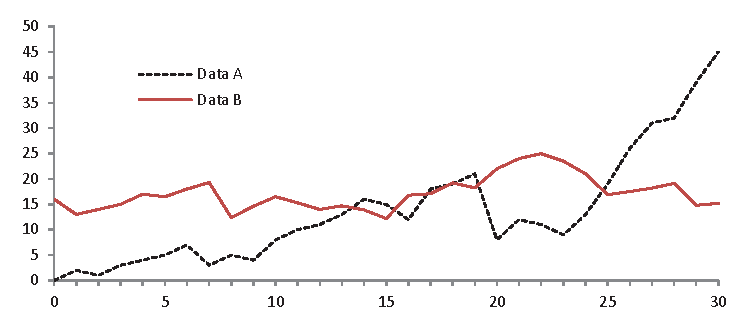
\includegraphics[width=\textwidth]{Figure/fig1.eps}
\caption{A figure caption is always placed below the illustration.
Please note that short captions are centered, while long ones are
justified by the macro package automatically.} \label{fig1}
\end{figure}

\begin{theorem}
This is a sample theorem. The run-in heading is set in bold, while
the following text appears in italics. Definitions, lemmas,
propositions, and corollaries are styled the same way.
\end{theorem}
%
% the environments 'definition', 'lemma', 'proposition', 'corollary',
% 'remark', and 'example' are defined in the LLNCS documentclass as well.
%
\begin{proof}
Proofs, examples, and remarks have the initial word in italics,
while the following text appears in normal font.
\end{proof}
For citations of references, we prefer the use of square brackets
and consecutive numbers. Citations using labels or the author/year
convention are also acceptable. The following bibliography provides
a sample reference list with entries for journal
articles~\cite{ref_article1}, an LNCS chapter~\cite{ref_lncs1}, a
book~\cite{ref_book1}, proceedings without editors~\cite{ref_proc1},
and a homepage~\cite{ref_url1}. Multiple citations are grouped
\cite{ref_article1,ref_lncs1,ref_book1},
\cite{ref_article1,ref_book1,ref_proc1,ref_url1}.
%
% ---- Bibliography ----
%
% BibTeX users should specify bibliography style 'splncs04'.
% References will then be sorted and formatted in the correct style.
%
% \bibliographystyle{splncs04}
% \bibliography{mybibliography}
%

\end{comment}

\begin{titlepage}
	\centering
	\includegraphics[width=0.15\textwidth]{UCLA.png}\par\vspace{1cm}
	\vspace{1cm}
	{\scshape\Large ECE219 Project 3 \par}
	\vspace{1.5cm}
	{\huge\bfseries Collaborative Filtering\par}
	\vspace{2cm}
	{\Large\itshape Zhilai~Shen, Yufei~Hu, Zheang~Huai, and Tianyi~Liu\par}
	{\Large\itshape 105023454, 404944367, 505222324, 705035425\par}
	\vfill

	\vfill

% Bottom of the page
	{\large \today\par}
\end{titlepage}

\tableofcontents

\newpage

\section{MovieLens dataset}

\bigbreak \textbf{Question 1:}

The sparsity of the movie rating dataset is: 0.017.
\newline

\bigbreak \textbf{Question 2:}

\begin{figure}
\centering
\scalebox{0.4}{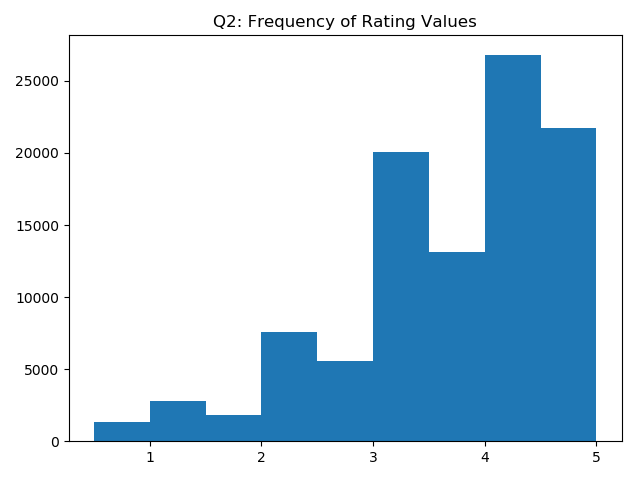
\includegraphics{Figure/Q2.png}}
\caption{Frequency of the rating values} \label{Q2}
\end{figure}

The shape of the histogram is skewed to the right. More higher ratings fall in 4 and 5 while ratings in 1 and 2 are rather lower.
\newline

\bigbreak \textbf{Question 3:}

\begin{figure}
\centering
\scalebox{0.4}{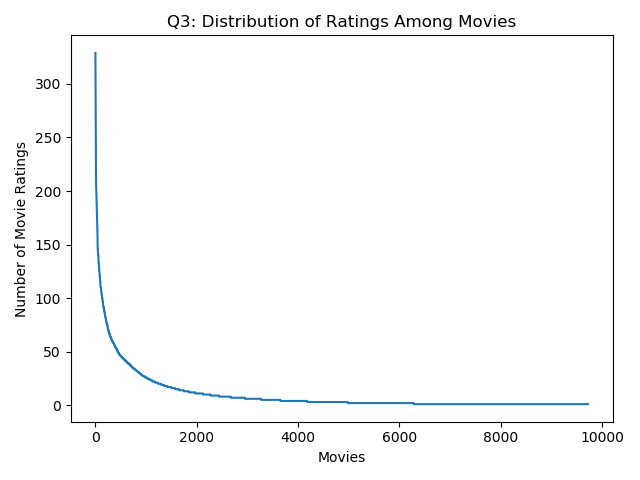
\includegraphics{Figure/Q3.png}}
\caption{Distribution of ratings among movies} \label{Q3}
\end{figure}

The distribution of the number of ratings received among movies can be seen in \ref{Q3}. A monotonically decreasing curve is observed.
\newline

\bigbreak \textbf{Question 4:}

\begin{figure}
\centering
\scalebox{0.4}{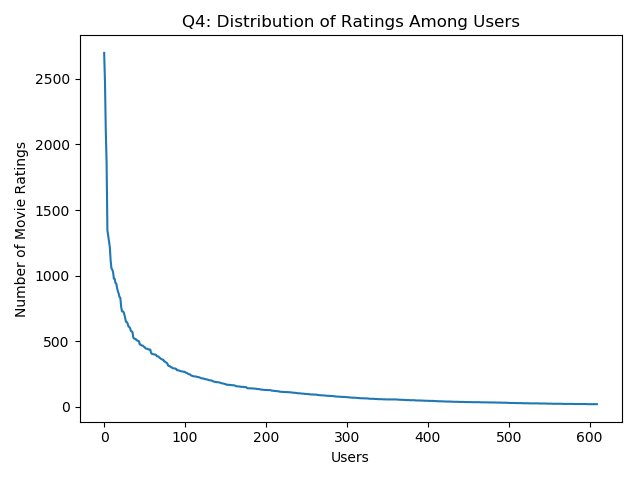
\includegraphics{Figure/Q4.png}}
\caption{Distribution of ratings among users} \label{Q4}
\end{figure}

The distribution of the number of ratings received among users can also be seen in \ref{Q4}. A monotonically decreasing curve is also observed.
\newline

\bigbreak \textbf{Question 5:}

As seen in \ref{Q3}, very few movies have more than 60 ratings, and most of the movies have fewer than 10 ratings. These features imply that the rating matrix is very sparse, which is the main challenge in the recommendation process as introduced in class. Also, about 500 movies have many ratings, meaning they are more popular compared to the rest of the movies.
\newline

\bigbreak \textbf{Question 6:}

\begin{figure}
\centering
\scalebox{0.4}{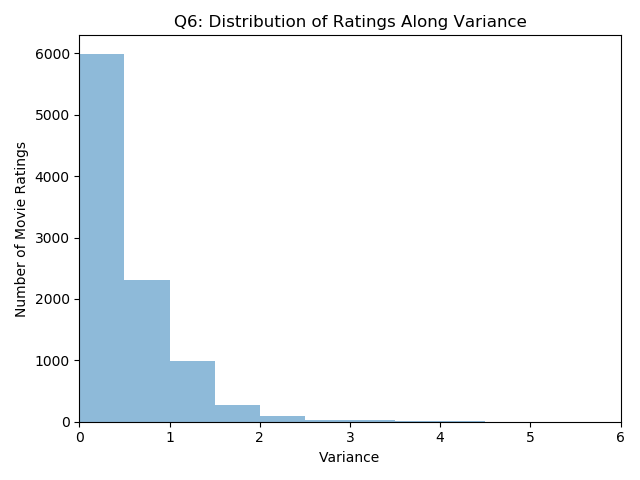
\includegraphics{Figure/Q6.png}}
\caption{Variance of the rating values received by each movie} \label{Q6}
\end{figure}

From \ref{Q6}, it is obversed that most of the movies receive similar ratings from users from the fact that their variances are less than 0.5. Very few movies have high variance of ratings among different users. This means that users have similar taste for most of the movies, which will ease the pain of designing our recommender system.
\newline

\section{Neighborhood-based collaborative filtering}

\subsection{Pearson-correlation coefficient}

\bigbreak \textbf{Question 7:}

\[\mu_u=\frac{1}{|I_u|}\sum_{k{\in}I_u} r_{uk}\]
\newline

\bigbreak \textbf{Question 8:}

${I_u}{\cap}{I_v}$ means the set of item indices for which ratings have been specified by both user v and u. It can be an empty set when none of the items rated by u has been rated by v and vise versa.
\newline

\subsection{Prediction function}

\bigbreak \textbf{Question 9:}

Mean-centering effectively produces user v's preference on item j compared to his average rating. For example, if user v tends to give high ratings, we could produce an unbiased rating by subtracting v's mean rating ${\mu}_{u}$ from actual rating.
\newline

\subsection{k-NN collaborative filter}

\subsubsection{Design and test via cross-validation}

\bigbreak \textbf{Question 10:}

\begin{figure}
\centering
\scalebox{0.4}{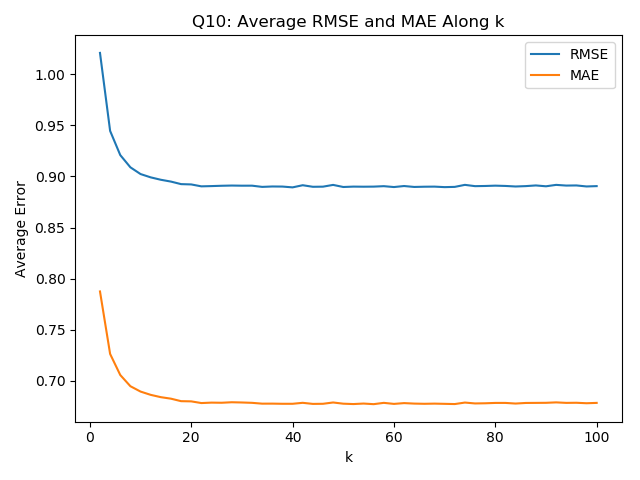
\includegraphics{Figure/Q10.png}}
\caption{Number of neighbors k against average MAE and RMSE} \label{Q10}
\end{figure}

The plot of the number of neighbors k vs average MAE and RMSE, for k = 2 to 100 can be seen in \ref{Q10}.
\newline

\bigbreak \textbf{Question 11:}
Minimum k of average RMSE is 22. Steady state values of average RMSE is 0.891. 
Minimum k of average MAE is 22. Steady state values of average MAE is 0.678. 


\subsection{Filter performance on trimmed test set}

\bigbreak \textbf{Question 12:}
\begin{figure}
\centering
\scalebox{0.7}{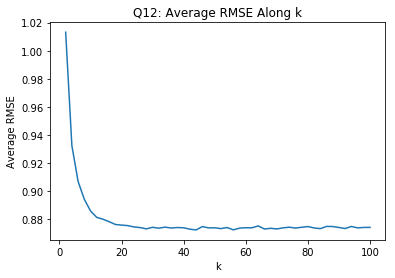
\includegraphics{Figure/Q12.png}}
\caption{average RMSE of popular movie trimmed test set} \label{Q12}
\end{figure}

The plot of average RMSE against k, for k = 2 to 100 can be seen in Figure \ref{Q12}.The minimum average RMSE is 0.8724.
\newline


\bigbreak \textbf{Question 13:}
\begin{figure}
\centering
\scalebox{0.7}{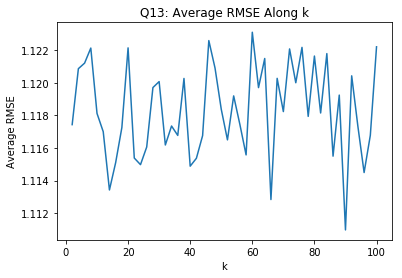
\includegraphics{Figure/Q13.png}}
\caption{average RMSE of unpopular movie trimmed test set} \label{Q13}
\end{figure}

The plot of average RMSE against k, for k = 2 to 100 can be seen in Figure \ref{Q13}.The minimum average RMSE is 1.1110.
\newline

\bigbreak \textbf{Question 14:}
\begin{figure}
\centering
\scalebox{0.7}{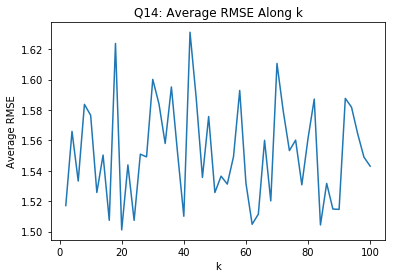
\includegraphics{Figure/Q14.png}}
\caption{average RMSE of high variance movie trimmed test set} \label{Q14}
\end{figure}

The plot of average RMSE against k, for k = 2 to 100 can be seen in Figure \ref{Q14}.The minimum average RMSE is 1.5011.
\newline

\subsubsection{Performance evaluation using ROC curve}

\bigbreak \textbf{Question 15:}
\begin{figure}
\centering
\scalebox{0.7}{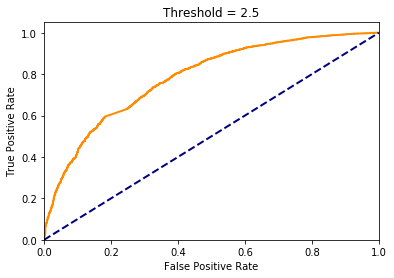
\includegraphics{Figure/Q15_1.png}}
\caption{ROC curve for the k-NN collaborative filter, threshold=2.5} \label{Q15_1}
\end{figure}

\begin{figure}
\centering
\scalebox{0.7}{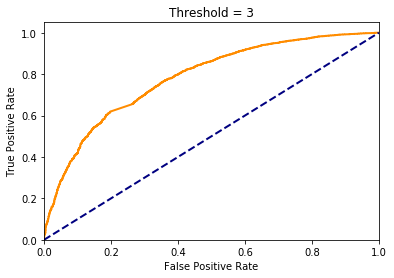
\includegraphics{Figure/Q15_2.png}}
\caption{ROC curve for the k-NN collaborative filter, threshold=3} \label{Q15_2}
\end{figure}

\begin{figure}
\centering
\scalebox{0.7}{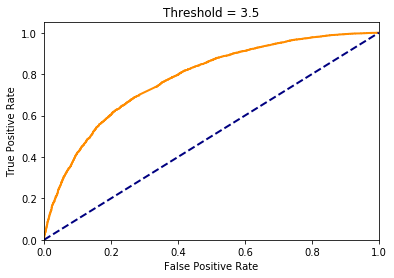
\includegraphics{Figure/Q15_3.png}}
\caption{ROC curve for the k-NN collaborative filter, threshold=3.5} \label{Q15_3}
\end{figure}

\begin{figure}
\centering
\scalebox{0.7}{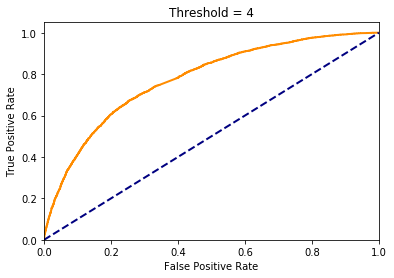
\includegraphics{Figure/Q15_4.png}}
\caption{ROC curve for the k-NN collaborative filter, threshold=4} \label{Q15_4}
\end{figure}

\begin{table}[h]
\center
\caption{AUC values of different thresholds}
\scalebox{0.9}{
\begin{tabular}{c|c}
\hline
threshold & AUC \\\hline
2.5 & 0.7828 \\\hline
3 & 0.7813 \\\hline
3.5 & 0.7798 \\\hline
4 & 0.7756\\\hline
\end{tabular}}
\label{tab:q15}
\end{table}

The ROC curves for different threshold values [2.5,3,3.5,4] can be seen in Figure \ref{Q15_1},Figure \ref{Q15_2},Figure \ref{Q15_3},Figure \ref{Q15_4}, respectively. The AUC values can be seen in Table \ref{tab:q15}.
\newline

\section{Model-based collaborative filtering}

\bigbreak \textbf{Question 16:}
The answer is in the picture below.

\begin{figure}
\scalebox{0.13}{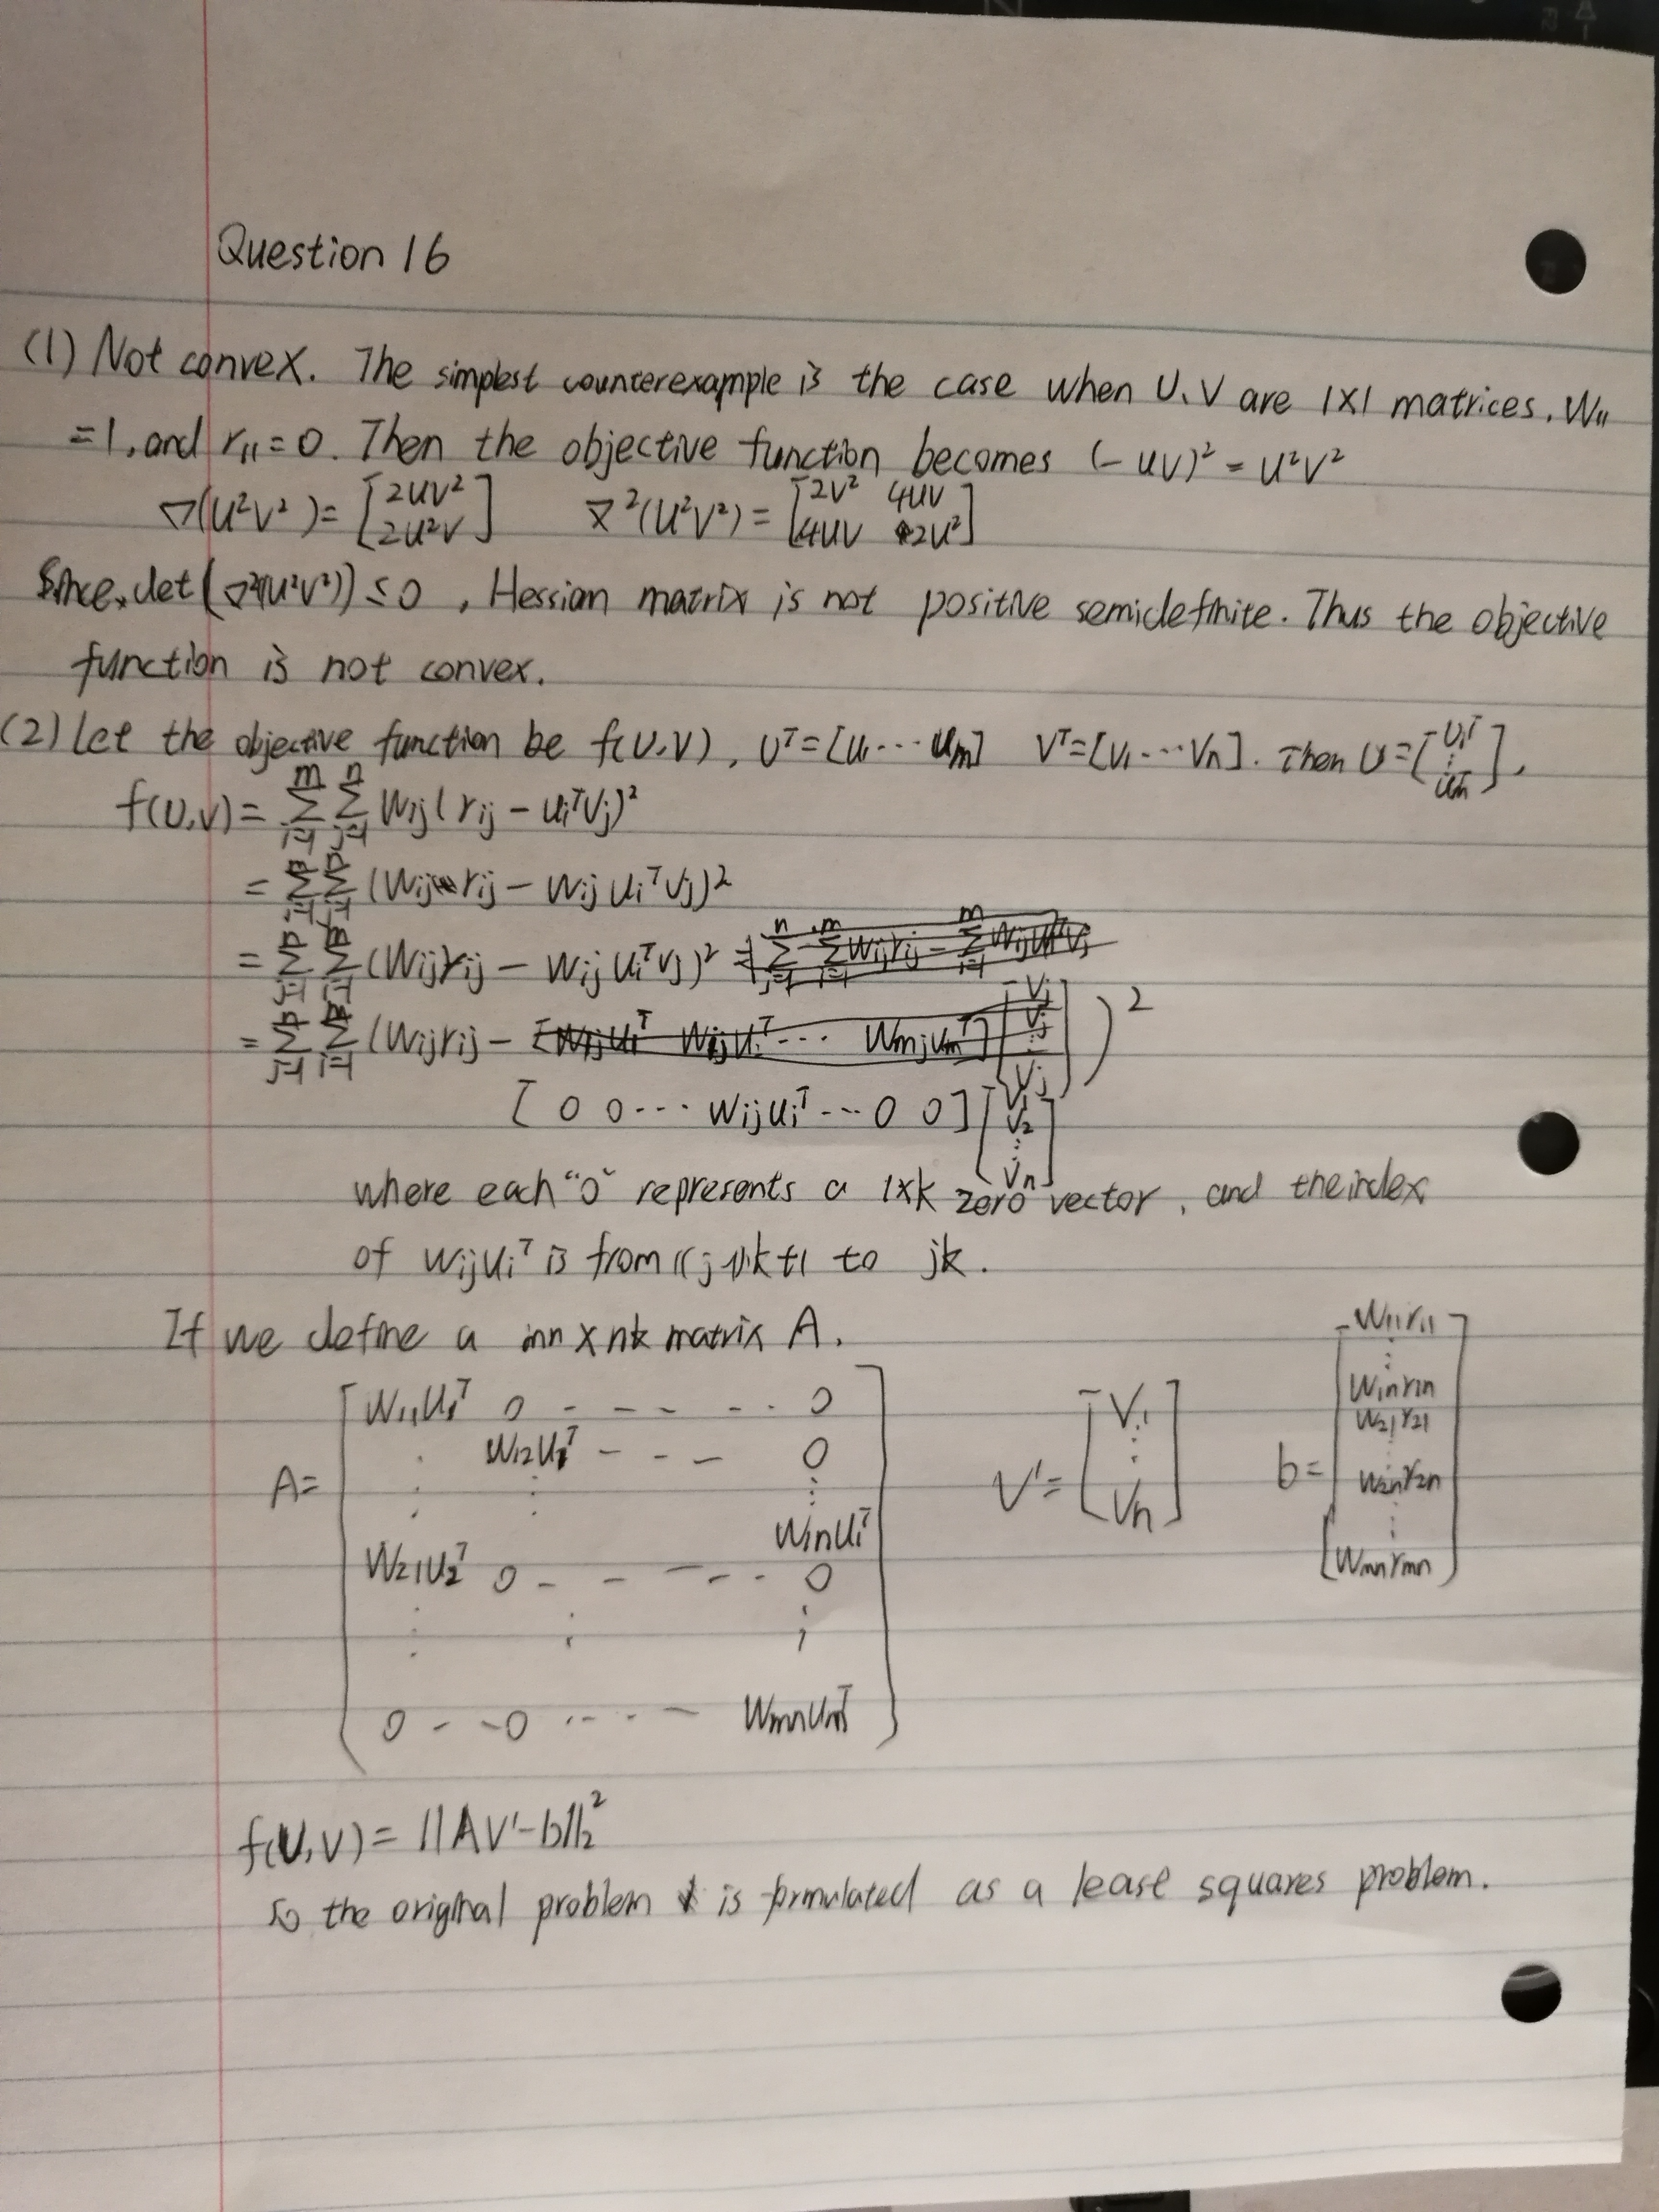
\includegraphics{Figure/Q16.png}}
\end{figure}

\subsubsection{Design and test via cross-validation}

\bigbreak \textbf{Question 17:}
\begin{figure}
\centering
\scalebox{0.7}{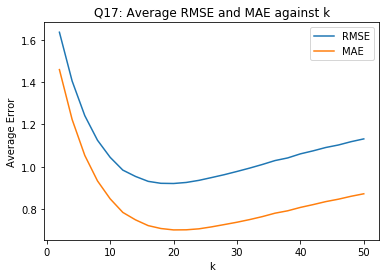
\includegraphics{Figure/Q17.png}}
\caption{Average RMSE and average MAE against k} \label{Q17}
\end{figure}

The plot of the average RMSE and the average MAE against k, for k = 2 to 50 can be seen in Figure \ref{Q17}.
\newline.

\bigbreak \textbf{Question 18:}
The optimal number of latent factors is 20. The minimum average RMSE and MAE are 0.9204, 0.7009, respectively. As can be seen in the readme file of dataset, there are 18 genres. So the optimal number of latent factors is not exactly the same as the number of movie genres but very close to the number of movie genres.
\newline

\subsubsection{NNMF filter performance on trimmed test set}

\bigbreak \textbf{Question 19:}
\begin{figure}
\centering
\scalebox{0.7}{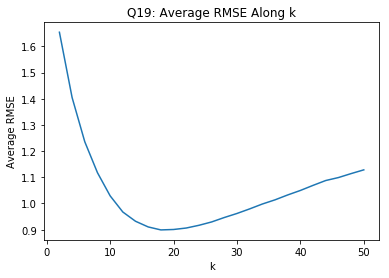
\includegraphics{Figure/Q19.png}}
\caption{Average RMSE of popular movie trimmed test set} \label{Q19}
\end{figure}

The plot of average RMSE against k, for k = 2 to 50 can be seen in Figure \ref{Q19}. The minimum average RMSE is 0.8991.
\newline

\bigbreak \textbf{Question 20:}
\begin{figure}
\centering
\scalebox{0.7}{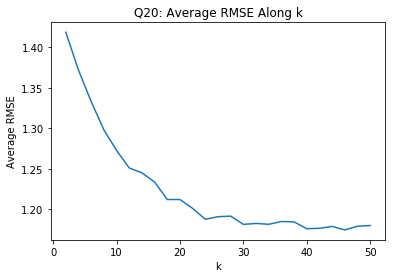
\includegraphics{Figure/Q20.png}}
\caption{Average RMSE of unpopular movie trimmed test set} \label{Q20}
\end{figure}

The plot of average RMSE against k, for k = 2 to 50 can be seen in Figure \ref{Q20}. The minimum average RMSE is 1.1748.
\newline

\bigbreak \textbf{Question 21:}
\begin{figure}
\centering
\scalebox{0.7}{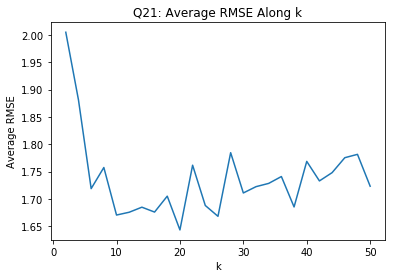
\includegraphics{Figure/Q21.png}}
\caption{Average RMSE of high variance movie trimmed test set} \label{Q21}
\end{figure}

The plot of average RMSE against k, for k = 2 to 50 can be seen in Figure \ref{Q21}. The minimum average RMSE is 1.6433.
\newline

\subsubsection{Performance evaluation using ROC curve}

\bigbreak \textbf{Question 22:}
The plots are as in Figure \ref{Q221}, \ref{Q222}, \ref{Q223}, \ref{Q224}.
\begin{figure}
\centering
\scalebox{0.7}{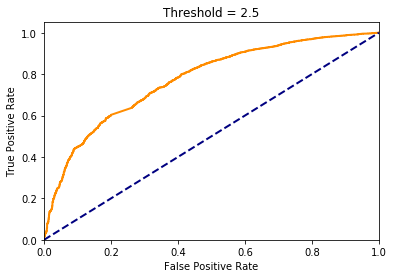
\includegraphics{Figure/Q22_1.png}}
\caption{ROC curve for the NNMF collaborative filter, threshold=2.5} \label{Q221}
\end{figure}

\begin{figure}
\centering
\scalebox{0.7}{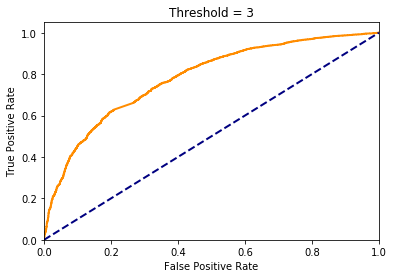
\includegraphics{Figure/Q22_2.png}}
\caption{ROC curve for the NNMF collaborative filter, threshold=3} \label{Q222}
\end{figure}

\begin{figure}
\centering
\scalebox{0.7}{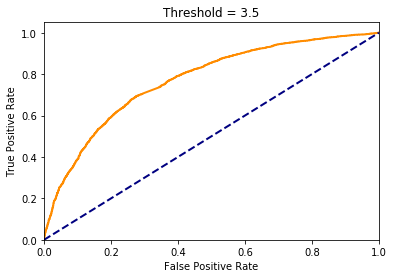
\includegraphics{Figure/Q22_3.png}}
\caption{ROC curve for the NNMF collaborative filter, threshold=3.5} \label{Q223}
\end{figure}

\begin{figure}
\centering
\scalebox{0.7}{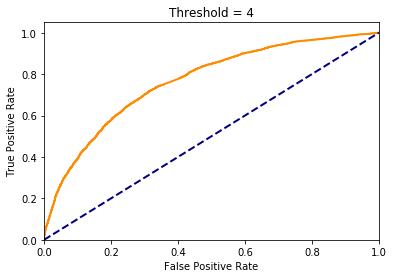
\includegraphics{Figure/Q22_4.png}}
\caption{ROC curve for the NNMF collaborative filter, threshold=4} \label{Q224}
\end{figure}

And the corresponding Area under Curve is in the table \ref{tab:Q22T}.

\begin{table}[h]
\center
\caption{AUC values of different thresholds}
\scalebox{0.9}{
\begin{tabular}{c|c}
\hline
threshold & AUC \\\hline
2.5 & 0.774 \\\hline
3 & 0.781 \\\hline
3.5 & 0.770 \\\hline
4 & 0.766\\\hline
\end{tabular}}
\label{tab:Q22T}
\end{table}


\subsubsection{Interpretability of NNMF}

\bigbreak \textbf{Question 23:}
Several columns are reported as following in table \ref{tab:Q22c1}, \ref{tab:Q22c2}, \ref{tab:Q22c3}, \ref{tab:Q22c4}, \ref{tab:Q22c5}. As can been seen from the tables, most of the movies belong to one particular collection of genres: comedy and drama. Also, there is connection between latent factors and movie genres. Since the rows and columns of the rating matrix are co-related, and high rating movies are usually people's most favorite movies. As a result, after sorting the latent matrix, we find that comedy, drama and romance are the three most welcomed genres. In the matrix, these are also three genres that rating the highest. 


\begin{table}[h]
\center
\caption{Top 10 movie for column 1}
\scalebox{0.9}{
\begin{tabular}{c|c}
\hline
movieID & genres \\\hline
3461 & Adventure|Drama|Thriller \\\hline
6201 & Drama|Romance \\\hline
5027 & Action|Comedy|Crime|Drama|Thriller \\\hline
74282 & Children|Drama|Romance\\\hline
2506 & Comedy|Drama|Romance \\\hline
177765 & Adventure|Animation|Children \\\hline
49272 & Action|Adventure|Thriller \\\hline
165483 & Comedy\\\hline
53161 & Comedy|Drama|Romance|Sci-Fi \\\hline
4178 & Drama\\\hline
\end{tabular}}
\label{tab:Q22c1}
\end{table}

\begin{table}[h]
\center
\caption{Top 10 movie for column 2}
\scalebox{0.9}{
\begin{tabular}{c|c}
\hline
movieID & genres \\\hline
2724 & Comedy|Romance \\\hline
100159 & Comedy \\\hline
26547 & Action|Comedy|Crime|Thriller \\\hline
62250 & Crime|Drama\\\hline
86781 & Drama|Mystery|War \\\hline
1643 & Drama|Romance \\\hline
72226 & Adventure|Animation|Children|Comedy|Crime \\\hline
71732 & Comedy|Horror\\\hline
184349 & Comedy|Drama|Romance \\\hline
414 & Comedy\\\hline
\end{tabular}}
\label{tab:Q22c2}
\end{table}

\begin{table}[h]
\center
\caption{Top 10 movie for column 3}
\scalebox{0.9}{
\begin{tabular}{c|c}
\hline
movieID & genres \\\hline
937 & Comedy|Romance \\\hline
4205 & Comedy|Drama|Romance \\\hline
61240 & Drama|Fantasy|Horror|Romance \\\hline
70183 & Comedy|Drama|Romance\\\hline
17 & Drama|Romance \\\hline
7932 & Documentary \\\hline
1356 & Action|Adventure|Sci-Fi|Thriller \\\hline
26777 & Drama\\\hline
5328 & Drama|Romance \\\hline
5849 & Comedy\\\hline
\end{tabular}}
\label{tab:Q22c3}
\end{table}

\begin{table}[h]
\center
\caption{Top 10 movie for column 4}
\scalebox{0.9}{
\begin{tabular}{c|c}
\hline
movieID & genres \\\hline
4619 & Comedy \\\hline
5016 & Drama \\\hline
183611 & Action|Comedy|Crime|Horror \\\hline
4849 & Comedy|Drama\\\hline
89745 & Action|Adventure|Sci-Fi|IMAX \\\hline
7299 & Drama \\\hline
56174 & Action|Horror|Sci-Fi|Thriller|IMAX \\\hline
114028 & Comedy|Drama\\\hline
136445 & Comedy \\\hline
4499 & Comedy\\\hline
\end{tabular}}
\label{tab:Q22c4}
\end{table}

\begin{table}[h]
\center
\caption{Top 10 movie for column 5}
\scalebox{0.9}{
\begin{tabular}{c|c}
\hline
movieID & genres \\\hline
27373 & Drama \\\hline
170355 & Drama|Mystery|Romance \\\hline
103810 & Action|Comedy|Crime|Thriller \\\hline
51834 & Drama|Romance\\\hline
3005 & Thriller \\\hline
32582 & Documentary \\\hline
84553 & Comedy \\\hline
2921 & Western\\\hline
80126 & Drama|Thriller \\\hline
52694 & Comedy\\\hline
\end{tabular}}
\label{tab:Q22c5}
\end{table}




\subsection{Matrix factorization with bias (MF with bias)}

\subsubsection{Design and test via cross-validation}

\bigbreak \textbf{Question 24:}
The RMSE and MSE plots against k is in the figure \ref{Q24}. As seen in the figure, when k = 26, it reaches minimum average RMSE and MSE.

\begin{figure}
\centering
\scalebox{0.7}{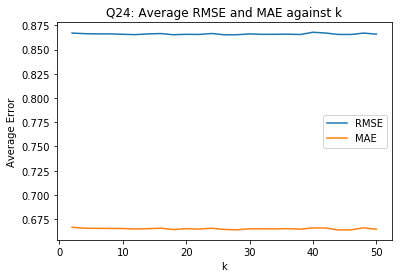
\includegraphics{Figure/Q24.png}}
\caption{Average RMSE and average MAE against k} \label{Q24}
\end{figure}


\bigbreak \textbf{Question 25:}
The optimal number of latent factors k is 26.

\subsubsection{MF with bias filter performance on trimmed test set}

\bigbreak \textbf{Question 26:}
The average RMSE against k is in figure \ref{Q26}. The minimum average RMSE is 0.857.

\begin{figure}
\centering
\scalebox{0.7}{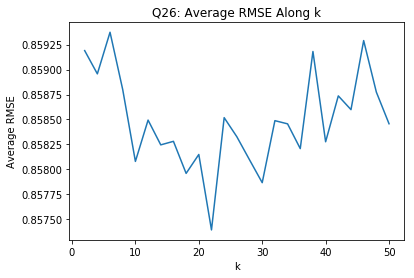
\includegraphics{Figure/Q26.png}}
\caption{Average RMSE against k} \label{Q26}
\end{figure}


\bigbreak \textbf{Question 27:}
The average RMSE against k is in figure \ref{Q27}. The minimum average RMSE is 0.971.

\begin{figure}
\centering
\scalebox{0.7}{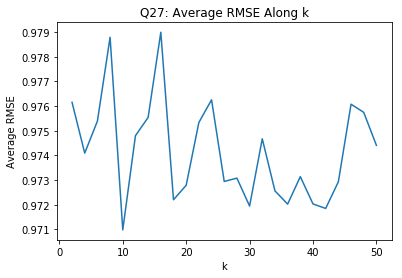
\includegraphics{Figure/Q27.png}}
\caption{Average RMSE against k} \label{Q27}
\end{figure}

\bigbreak \textbf{Question 28:}
The average RMSE against k is in figure \ref{Q28}. The minimum average RMSE is 1.435.

\begin{figure}
\centering
\scalebox{0.7}{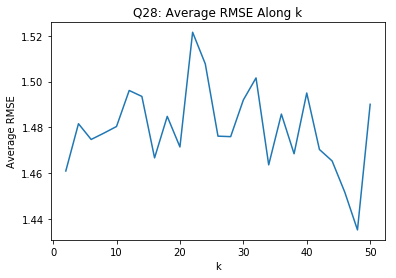
\includegraphics{Figure/Q28.png}}
\caption{Average RMSE against k} \label{Q28}
\end{figure}

\subsubsection{Performance evaluation using ROC curve}

\bigbreak \textbf{Question 29:}
The plots are as in Figure \ref{Q291}, \ref{Q292}, \ref{Q293}, \ref{Q294}.
\begin{figure}
\centering
\scalebox{0.7}{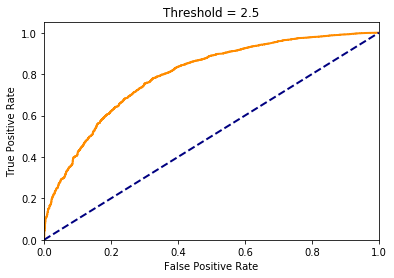
\includegraphics{Figure/Q29_1.png}}
\caption{ROC curve for the MF collaborative filter with bias, threshold=2.5} \label{Q291}
\end{figure}

\begin{figure}
\centering
\scalebox{0.7}{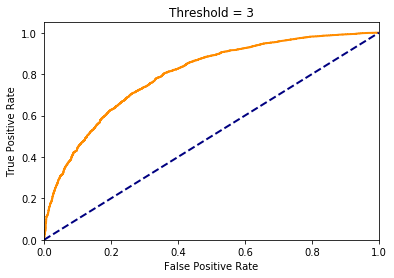
\includegraphics{Figure/Q29_2.png}}
\caption{ROC curve for the MF collaborative filter with bias, threshold=3} \label{Q292}
\end{figure}

\begin{figure}
\centering
\scalebox{0.7}{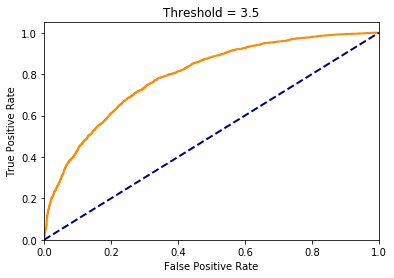
\includegraphics{Figure/Q29_3.png}}
\caption{ROC curve for the MF collaborative filter with bias, threshold=3.5} \label{Q293}
\end{figure}

\begin{figure}
\centering
\scalebox{0.7}{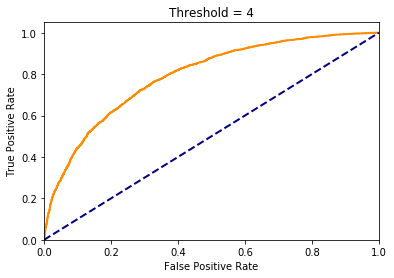
\includegraphics{Figure/Q29_4.png}}
\caption{ROC curve for the MF collaborative filter with bias, threshold=4} \label{Q294}
\end{figure}

And the corresponding Area under Curve is in the table \ref{tab:Q29T}.

\begin{table}[h]
\center
\caption{AUC values of different thresholds}
\scalebox{0.9}{
\begin{tabular}{c|c}
\hline
threshold & AUC \\\hline
2.5 & 0.794 \\\hline
3 & 0.797 \\\hline
3.5 & 0.792 \\\hline
4 & 0.791\\\hline
\end{tabular}}
\label{tab:Q29T}
\end{table}




\section{Naive collaborative filtering}

\subsection{Design and test via cross-validation}

\bigbreak \textbf{Question 30:}

We designed a naive collaborative filter to predict the ratings of the movies and the average RMSE by averaging the RMSE across all 10 folds is $0.9347$.

\subsection{Naive collaborative filter performance on trimmed test set}

\bigbreak \textbf{Question 31:}

Now we will test the performance of the filter in predicting the ratings of the movies in the trimmed test set. The average RMSE for popular movies is $0.9323$. The accuracy is a little bit higher than original dataset, which can be explained as there's more similarities in popular movies (that's why it's called popular movie).

\bigbreak \textbf{Question 32:}

The average RMSE for unpopular movies is $0.9323$. The accuracy is a little bit lower than original dataset. As far as I am concerned, it's the same reason as the popular movies.

\bigbreak \textbf{Question 33:}

The average RMSE for high variance movies is $1.4716$. The performance for high variance movies is even worse. But it's pretty obvious because it's high variance, it's very hard to detect the similarities between those movies and predict very well.


\section{Performance comparison}

\bigbreak \textbf{Question 34:}

The ROC curves (threshold = $3$) for the k-NN, NNMF, and MF with bias based collaborative filters is shown in Figure \ref{Q34}. We could see from the ROC curve that all those different methods give us pretty same results and it means that those model have similar performance. But if we have to choose the best one, MF collective filter seems like a little bit better.

\begin{figure}
\centering
\scalebox{0.5}{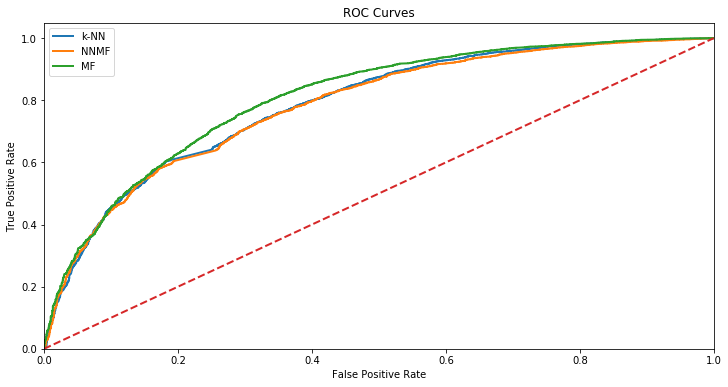
\includegraphics{Figure/Q34.png}}
\caption{The ROC curves for the k-NN, NNMF, and MF} 
\label{Q34}
\end{figure}


\section{Ranking}

\subsection{Evaluating ranking using precision-recall curve}

\bigbreak \textbf{Question 35:}

Precision is the ratio of correctly predicted positive observations to the total predicted positive observations. High precision relates to the low false positive rate. In the recommendation system it represents the fraction of recommended items that are correct or liked by users.

On the other hand,  recall is the ratio of correctly predicted positive observations to the all observations in actual class. It's basically the fraction of liked items that come from recommendation system.

\bigbreak \textbf{Question 36:}

The plot of average precision against size for the ranking obtained using k-NN collaborative filter predictions with $k = 22$ is shown in Figure \ref{Q361}. Also, the plot the average recall against size and average precision against average recall are Figure \ref{Q362} and \ref{Q363}.

We can see from those plots that as the number of the recommendations increases, the precision becomes lower and lower and the recall becomes higher and higher on the contrary. This phenomenon can be also observed from the plot of the precision against recall, which is pretty obvious that if you recommend more and more, you are more likely to recommend what users like but you can not guarantee the precision of your recommendation at the same time. It's a tradeoff.

\begin{figure}
\centering
\scalebox{0.5}{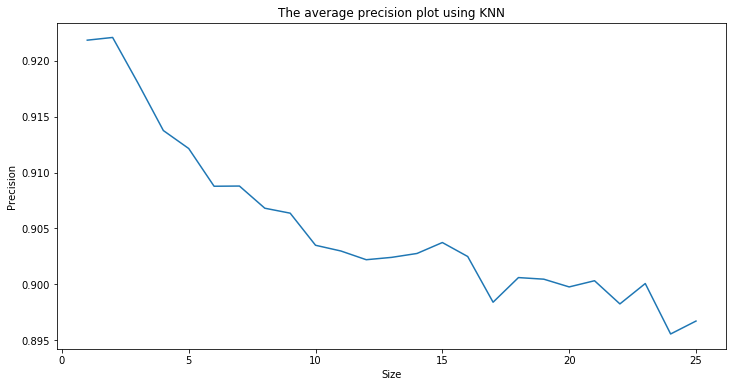
\includegraphics{Figure/Q36_1.png}}
\caption{The average precision against size for the k-NN} 
\label{Q361}
\end{figure}

\begin{figure}
\centering
\scalebox{0.5}{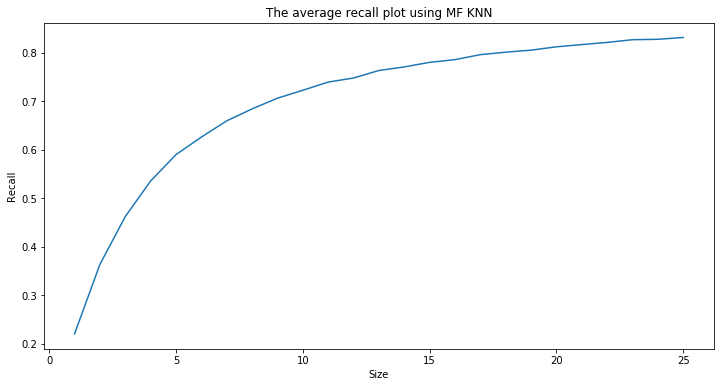
\includegraphics{Figure/Q36_2.png}}
\caption{The average recall against size for the k-NN} 
\label{Q362}
\end{figure}

\begin{figure}
\centering
\scalebox{0.5}{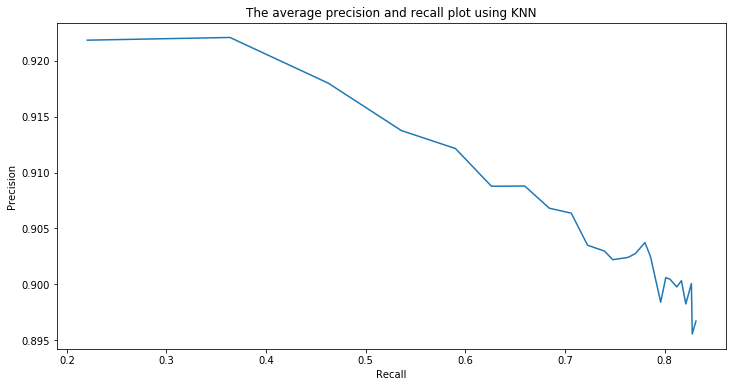
\includegraphics{Figure/Q36_3.png}}
\caption{The average precision against recall for the k-NN} 
\label{Q363}
\end{figure}

\bigbreak \textbf{Question 37:}

Similarly, the plot of average precision against size for the ranking obtained using NNMF collaborative filter predictions with $k = 20$ is shown in Figure \ref{Q371}. Also, the plot the average recall against size and average precision against average recall are Figure \ref{Q372} and \ref{Q373}.

The shape of the plots follow the same trends that we discuss previously. As the number of the recommendations increases, the precision goes down but the recall goes up.

\begin{figure}
\centering
\scalebox{0.5}{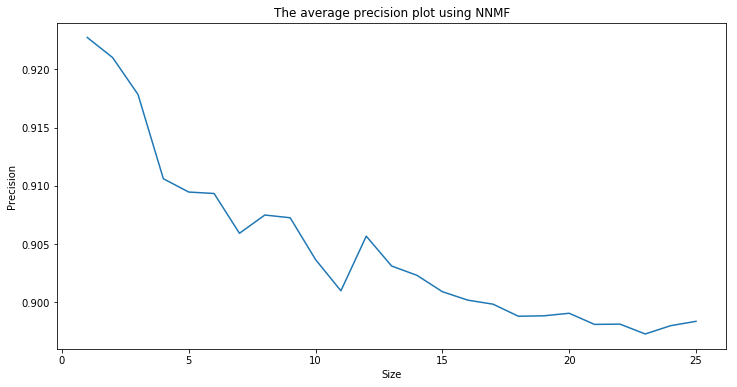
\includegraphics{Figure/Q37_1.png}}
\caption{The average precision against size for the NNMF} 
\label{Q371}
\end{figure}

\begin{figure}
\centering
\scalebox{0.5}{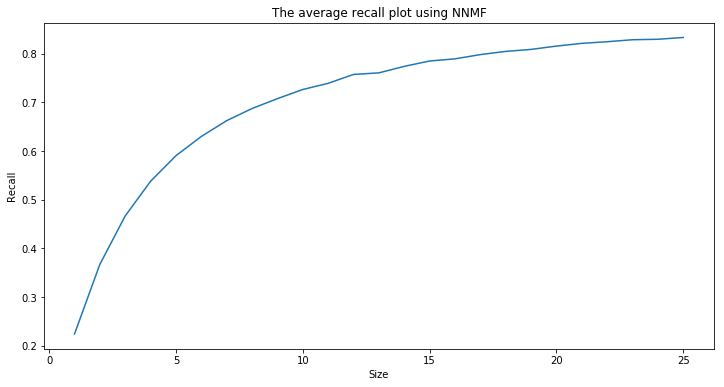
\includegraphics{Figure/Q37_2.png}}
\caption{The average recall against size for the NNMF} 
\label{Q372}
\end{figure}

\begin{figure}
\centering
\scalebox{0.5}{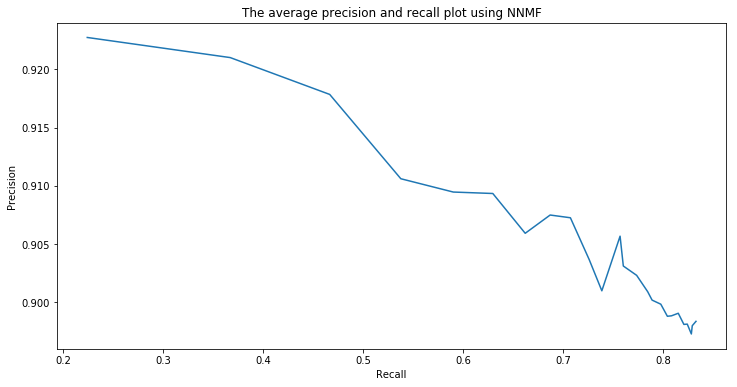
\includegraphics{Figure/Q37_3.png}}
\caption{The average precision against recall for the NNMF} 
\label{Q373}
\end{figure}

\bigbreak \textbf{Question 38:}

Same here, the plot of average precision against size for the ranking obtained using MF collaborative filter predictions with $k = 26$ is shown in Figure \ref{Q381}. Also, the plot the average recall against size and average precision against average recall are Figure \ref{Q382} and \ref{Q383}.

The shape of the plots are basically still the same.follow the same trends that we discuss previously. The precision and recall go to the contradictory direction   when the size growing.


\begin{figure}
\centering
\scalebox{0.5}{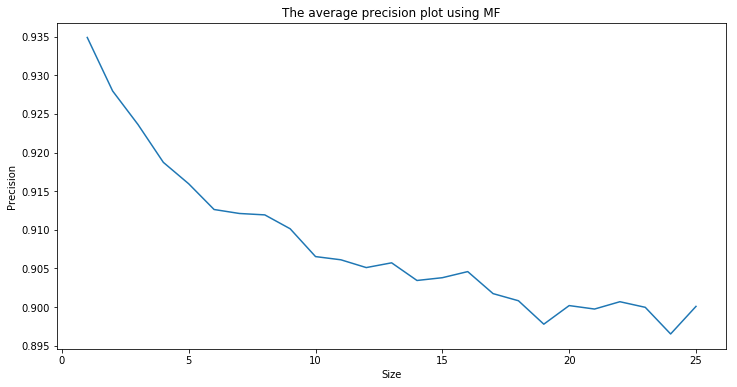
\includegraphics{Figure/Q38_1.png}}
\caption{The average precision against size for the MF} 
\label{Q381}
\end{figure}

\begin{figure}
\centering
\scalebox{0.5}{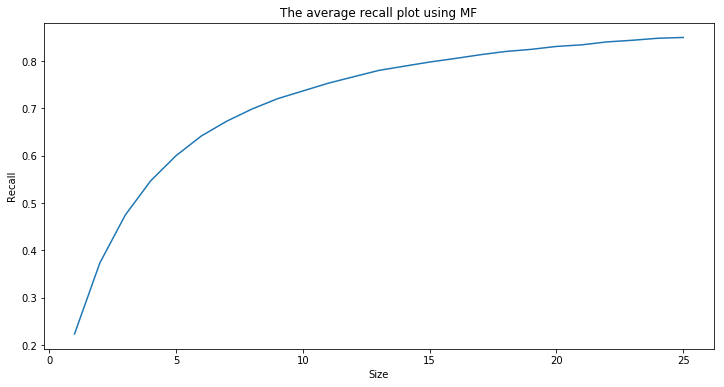
\includegraphics{Figure/Q38_2.png}}
\caption{The average recall against size for the MF} 
\label{Q382}
\end{figure}

\begin{figure}
\centering
\scalebox{0.5}{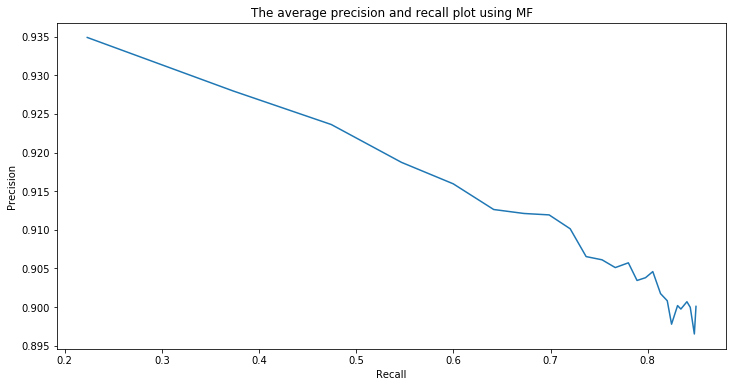
\includegraphics{Figure/Q38_3.png}}
\caption{The average precision against recall for the MF} 
\label{Q383}
\end{figure}

\bigbreak \textbf{Question 39:}

The precision-recall curves for the k-NN, NNMF, and MF with bias based collaborative filters is shown in Figure \ref{Q39}. We could see that in comparison to other two methods, MF collective filter got the best performance with higher precision and recall. But overall all three methods give us similar performance.

\begin{figure}
\centering
\scalebox{0.5}{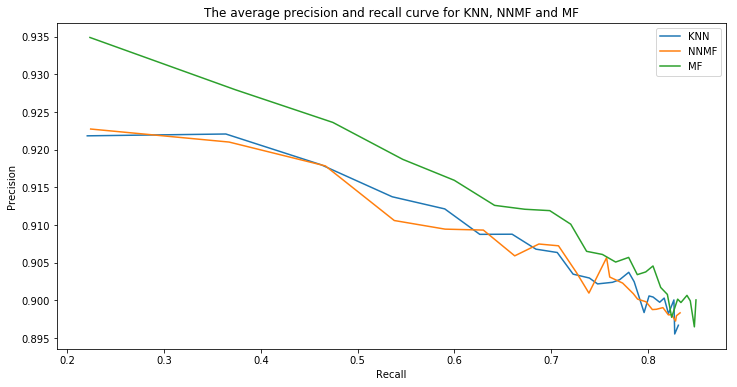
\includegraphics{Figure/Q39.png}}
\caption{The precision-recall curves for the k-NN, NNMF, and MF} 
\label{Q39}
\end{figure}

\end{document}
